\documentclass[twoside]{article}\usepackage[]{graphicx}\usepackage[]{color}
%% maxwidth is the original width if it is less than linewidth
%% otherwise use linewidth (to make sure the graphics do not exceed the margin)
\makeatletter
\def\maxwidth{ %
  \ifdim\Gin@nat@width>\linewidth
    \linewidth
  \else
    \Gin@nat@width
  \fi
}
\makeatother

\definecolor{fgcolor}{rgb}{0.345, 0.345, 0.345}
\newcommand{\hlnum}[1]{\textcolor[rgb]{0.686,0.059,0.569}{#1}}%
\newcommand{\hlstr}[1]{\textcolor[rgb]{0.192,0.494,0.8}{#1}}%
\newcommand{\hlcom}[1]{\textcolor[rgb]{0.678,0.584,0.686}{\textit{#1}}}%
\newcommand{\hlopt}[1]{\textcolor[rgb]{0,0,0}{#1}}%
\newcommand{\hlstd}[1]{\textcolor[rgb]{0.345,0.345,0.345}{#1}}%
\newcommand{\hlkwa}[1]{\textcolor[rgb]{0.161,0.373,0.58}{\textbf{#1}}}%
\newcommand{\hlkwb}[1]{\textcolor[rgb]{0.69,0.353,0.396}{#1}}%
\newcommand{\hlkwc}[1]{\textcolor[rgb]{0.333,0.667,0.333}{#1}}%
\newcommand{\hlkwd}[1]{\textcolor[rgb]{0.737,0.353,0.396}{\textbf{#1}}}%

\usepackage{framed}
\makeatletter
\newenvironment{kframe}{%
 \def\at@end@of@kframe{}%
 \ifinner\ifhmode%
  \def\at@end@of@kframe{\end{minipage}}%
  \begin{minipage}{\columnwidth}%
 \fi\fi%
 \def\FrameCommand##1{\hskip\@totalleftmargin \hskip-\fboxsep
 \colorbox{shadecolor}{##1}\hskip-\fboxsep
     % There is no \\@totalrightmargin, so:
     \hskip-\linewidth \hskip-\@totalleftmargin \hskip\columnwidth}%
 \MakeFramed {\advance\hsize-\width
   \@totalleftmargin\z@ \linewidth\hsize
   \@setminipage}}%
 {\par\unskip\endMakeFramed%
 \at@end@of@kframe}
\makeatother

\definecolor{shadecolor}{rgb}{.97, .97, .97}
\definecolor{messagecolor}{rgb}{0, 0, 0}
\definecolor{warningcolor}{rgb}{1, 0, 1}
\definecolor{errorcolor}{rgb}{1, 0, 0}
\newenvironment{knitrout}{}{} % an empty environment to be redefined in TeX

\usepackage{alltt}

\setlength{\oddsidemargin}{5mm}
\setlength{\evensidemargin}{5mm}
\usepackage{multicol}

\usepackage{fancyhdr}
\pagestyle{fancy}
\fancyheadoffset{0cm}
\fancyhead[LE,RO]{\thepage}
\cfoot{Confidential report for quality improvement purposes}

\renewcommand{\headrulewidth}{0.4pt}
\renewcommand{\footrulewidth}{0.4pt}

\usepackage[letterpaper]{geometry}
\geometry{hmarginratio=1:1}
\usepackage{amsfonts}
\usepackage{hyperref}
\hypersetup{
    colorlinks,
    citecolor=black,
    filecolor=black,
    linkcolor=black,
    urlcolor=black
}
%\renewcommand\footnotetext{}  % removes the footnote number
\renewcommand{\abstractname}{\vspace{-\baselineskip}}
\renewcommand{\familydefault}{\sfdefault}


\title{Pediatric and Neonatal Critical Care Transport Quality Metrics}
\date{2013 Cumulative Report}
\IfFileExists{upquote.sty}{\usepackage{upquote}}{}
\begin{document}
\maketitle
\thispagestyle{empty}

\begin{abstract}
This demonstration report is based on incomplete data for the year. In each of the graphs that follow, the vertical line shows the overall combined rate for all progams. The dots reflect the rate for each program and the horizontal bars indicate the 95\% confidence interval. When the horizontal bar does not cross the vertical line, this indicates that program's rate is significantly higher or lower than the overall rate.\\
\emph{Generated: \date{\today}}

\end{abstract}

\tableofcontents{}




\newpage
\section{Introduction}
This report is designed to give representation of a high-level cumulative overview of the individual institutional performance related to the included quality metrics.  As we`ve discussed, quality improvement run charts will be included in a separate report and are designed to present performance over time which is the optimal way to monitor these quality data on a continual basis.\\

Included in this report are the 12 “national” consensus metrics.  Reports for the remaining Ohio Collaborative metrics will be generated separately.  You`ll notice that there are some areas where we suspect that the “detection” of events is not sensitive (ex. medication administration errors) which is likely to afford us the opportunity as a collaborative to build the right detection/reporting mechanism. \\

Lastly, please remember that these data are de-identified, though there may be examples where you`ll be able to “infer” which program identifier is associated with which program.  There are no formal data-sharing agreements in place, though it is the expectation that these data should be solely used for quality improvement of critical care transport – both locally and nationally.  Performance data should not be used for marketing one program versus another.\\

\begin{multicols}{2}

  Michael T Bigham, MD, FAAP\\
  \\
  Pediatric Intensivist, Division of Critical Care Medicine\\
  Medical Director, Transport Services\\
  Assistant Patient Safety Officer\\
  Clinical Assistant Professor, NEOMED\\
  \url{mbigham@chmca.org}


Hamilton P. Schwartz, MD\\
\\
Medical Director, Statline\\
Medical Director, Pediatric Transport Program\\
Assistant Professor, UC Department of Pediatrics\\
\url{hamilton.schwartz@cchmc.org}\\

\end{multicols}

\newpage
\subsection*{Program Name - ID crosswalk}
% latex table generated in R 3.0.2 by xtable 1.7-1 package
% Fri May 30 21:10:43 2014
\begin{table}[ht]
\centering
\begin{tabular}{llr}
  \hline
ID & program\_name & total\_patients \\ 
  \hline
A & Memorial Childrens &  \\ 
  B & Yale-New Haven Childrens Neo &  \\ 
  C & Childrens WI & 264 \\ 
  D & Kentucky Childrens & 651 \\ 
  E & Nemours Childrens & 1061 \\ 
  F & LifeFlight of Maine &  \\ 
  G & Akron Childrens & 1994 \\ 
  H & St Vincent CCT &  \\ 
  I & Medical City Dallas &  \\ 
  J & Mattel Childrens &  \\ 
  K & Cardinal Glennon Childrens & 1184 \\ 
  L & Cincinnati Childrens & 1665 \\ 
  M & Kaiser Santa Clara &  \\ 
  N & Brenner Childrens &  \\ 
  O & Nationwide Childrens & 2025 \\ 
  P & Mercy Kids &  \\ 
  Q & Cleveland Clinic Childrens & 884 \\ 
  R & Texas Childrens & 1521 \\ 
  S & BC EHS &  \\ 
  T & Dell Childrens & 256 \\ 
  U & Childrens Kings Daughters &  \\ 
  V & Yale-New Haven Childrens Peds &  \\ 
  W & Air St Lukes &  \\ 
  X & Dayton Childrens & 3318 \\ 
  Y & Airlink & 20 \\ 
   \hline
\end{tabular}
\end{table}






%\let\thefootnote\relax\footnote{n = number of elligible cases (denominator)}
%\let\thefootnote\relax\footnote{k = number of cases of interest (numerator)}
%\let\thefootnote\relax\footnote{est = estimated percentage}
%\let\thefootnote\relax\footnote{lower/upper = lower \& upper 95\% confidence intervals}


\newpage
\section{Clinical metrics}
\subsection{Unintended neonatal hypothermia upon arrival to destination}
The number of neonates (infants less than 28 days) with admission temperatures at the destination facility less than 36.5 C axillary (excluding those being actively cooled) DIVIDED by the number of neonates transported during the calendar month.

\begin{center}
\begin{knitrout}
\definecolor{shadecolor}{rgb}{0.969, 0.969, 0.969}\color{fgcolor}
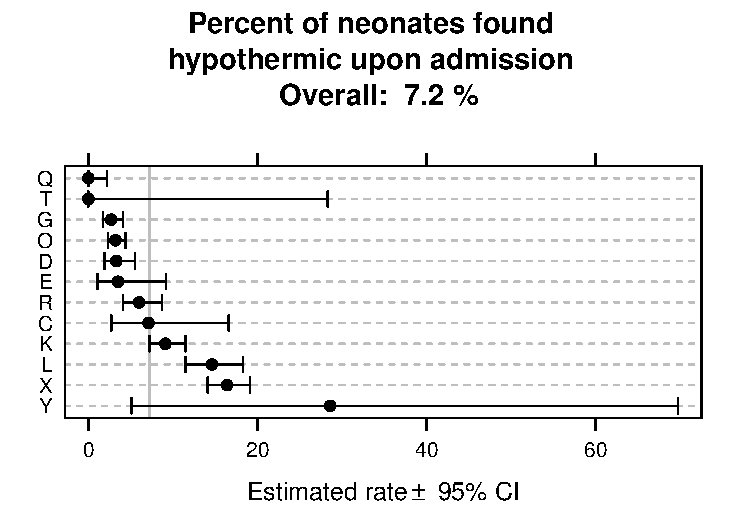
\includegraphics[width=\maxwidth]{figure/r_neonatal_hypothermia} 

\end{knitrout}

\end{center}

% latex table generated in R 3.0.2 by xtable 1.7-1 package
% Fri May 30 21:10:44 2014
\begin{table}[ht]
\centering
\begin{tabular}{lrrrrr}
  \hline
Program & den. & num. & lower CI & rate & upper CI \\ 
  \hline
Q & 217.0 & 0.0 & 0.0 & 0.0 & 2.2 \\ 
  T & 13.0 & 0.0 & 0.0 & 0.0 & 28.3 \\ 
  G & 858.0 & 23.0 & 1.7 & 2.7 & 4.1 \\ 
  O & 1163.0 & 37.0 & 2.3 & 3.2 & 4.4 \\ 
  D & 454.0 & 15.0 & 1.9 & 3.3 & 5.5 \\ 
  E & 115.0 & 4.0 & 1.1 & 3.5 & 9.2 \\ 
  R & 450.0 & 27.0 & 4.1 & 6.0 & 8.7 \\ 
  C & 70.0 & 5.0 & 2.7 & 7.1 & 16.6 \\ 
  K & 722.0 & 66.0 & 7.2 & 9.1 & 11.5 \\ 
  L & 446.0 & 65.0 & 11.5 & 14.6 & 18.3 \\ 
  X & 876.0 & 144.0 & 14.1 & 16.4 & 19.1 \\ 
  Y & 7.0 & 2.0 & 5.1 & 28.6 & 69.7 \\ 
   \hline
\end{tabular}
\end{table}




\newpage
\subsection{Verification of tracheal tube placement}
The number of tracheal tubes (TT) on transport (regardless of whether or not the transport team placed them themselves) for which there is documentation confirming placement using a minimum of 2 of the following confirmatory techniques: x-ray, direct visualization through the cords, continuous capnometry, or use of a colorimetric capnometer, and assessment for symetric breath sounds DIVIDED by the number of intubated patients transported during the calendar month.

\begin{center}
\begin{knitrout}
\definecolor{shadecolor}{rgb}{0.969, 0.969, 0.969}\color{fgcolor}
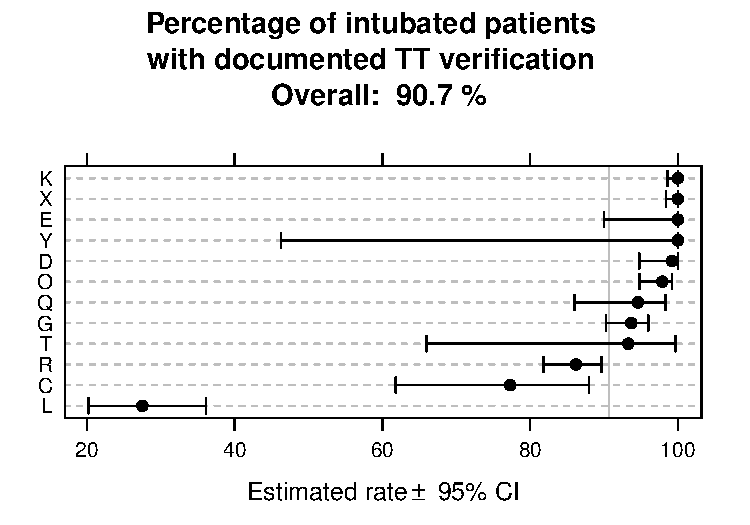
\includegraphics[width=\maxwidth]{figure/r_tracheal_tube_placement} 

\end{knitrout}

\end{center}

% latex table generated in R 3.0.2 by xtable 1.7-1 package
% Fri May 30 21:10:44 2014
\begin{table}[ht]
\centering
\begin{tabular}{lrrrrr}
  \hline
Program & den. & num. & lower CI & rate & upper CI \\ 
  \hline
K & 335.0 & 335.0 & 98.6 & 100.0 & 100.0 \\ 
  X & 298.0 & 298.0 & 98.4 & 100.0 & 100.0 \\ 
  E & 44.0 & 44.0 & 90.0 & 100.0 & 100.0 \\ 
  Y & 5.0 & 5.0 & 46.3 & 100.0 & 100.0 \\ 
  D & 121.0 & 120.0 & 94.8 & 99.2 & 100.0 \\ 
  O & 234.0 & 229.0 & 94.8 & 97.9 & 99.2 \\ 
  Q & 74.0 & 70.0 & 86.0 & 94.6 & 98.3 \\ 
  G & 318.0 & 298.0 & 90.3 & 93.7 & 96.0 \\ 
  T & 15.0 & 14.0 & 66.0 & 93.3 & 99.7 \\ 
  R & 318.0 & 274.0 & 81.8 & 86.2 & 89.7 \\ 
  C & 44.0 & 34.0 & 61.8 & 77.3 & 88.0 \\ 
  L & 131.0 & 36.0 & 20.2 & 27.5 & 36.1 \\ 
   \hline
\end{tabular}
\end{table}




\newpage
\subsection{Unplanned dislodgement of therapeutic devices}
The number of documented dislodgements (may be more than 1 per tansport) while under the care of the transport team of the following devices (IOs, IVs, UACs/UVCs, central venous lines, arterial lines, tracheal tubes, chest tubes, and tracheostomy tubes) DIVIDED by the number of transports during the calendar month. This does not include IVs that infiltrate without obvious dislodgement.

\begin{center}
\begin{knitrout}
\definecolor{shadecolor}{rgb}{0.969, 0.969, 0.969}\color{fgcolor}
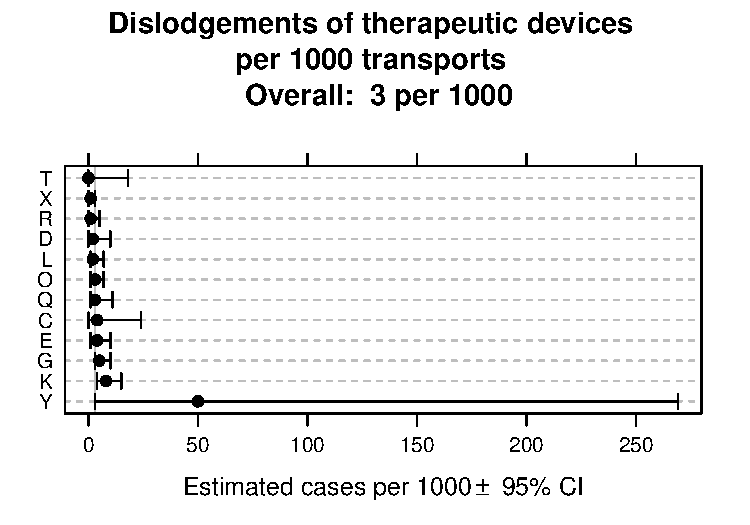
\includegraphics[width=\maxwidth]{figure/r_unplanned_dislodgement} 

\end{knitrout}

\end{center}

% latex table generated in R 3.0.2 by xtable 1.7-1 package
% Fri May 30 21:10:44 2014
\begin{table}[ht]
\centering
\begin{tabular}{lrrrrr}
  \hline
Program & den. & num. & lower CI & rate & upper CI \\ 
  \hline
T & 256.0 & 0.0 & 0.0 & 0.0 & 18.0 \\ 
  X & 3318.0 & 4.0 & 0.0 & 1.0 & 3.0 \\ 
  R & 1521.0 & 2.0 & 0.0 & 1.0 & 5.0 \\ 
  D & 651.0 & 1.0 & 0.0 & 2.0 & 10.0 \\ 
  L & 1665.0 & 4.0 & 1.0 & 2.0 & 7.0 \\ 
  O & 2025.0 & 6.0 & 1.0 & 3.0 & 7.0 \\ 
  Q & 884.0 & 3.0 & 1.0 & 3.0 & 11.0 \\ 
  C & 264.0 & 1.0 & 0.0 & 4.0 & 24.0 \\ 
  E & 1061.0 & 4.0 & 1.0 & 4.0 & 10.0 \\ 
  G & 1994.0 & 10.0 & 3.0 & 5.0 & 10.0 \\ 
  K & 1184.0 & 9.0 & 4.0 & 8.0 & 15.0 \\ 
  Y & 20.0 & 1.0 & 3.0 & 50.0 & 269.0 \\ 
   \hline
\end{tabular}
\end{table}



\newpage
\subsection{Neonatal: First attempt tracheal tube placement success}
The total number of intubations successful on the first attempt DIVIDED by the number of patients on whom intubation was attempted by the transport team during the calendar month. "Intubation attempt" is further defined as laryngoscopy by any member of the transport team regardless of whether there is an attempt to pass a tracheal tube. A successful intubation is further defined as that which has been confirmed as described in "Verification of TT tube placement." First-attempt success should not be disqualified by necessary adjustments to the depth of the TT and re-securing it. Includes patients less than 28 days (neonates).

\begin{center}
\begin{knitrout}
\definecolor{shadecolor}{rgb}{0.969, 0.969, 0.969}\color{fgcolor}
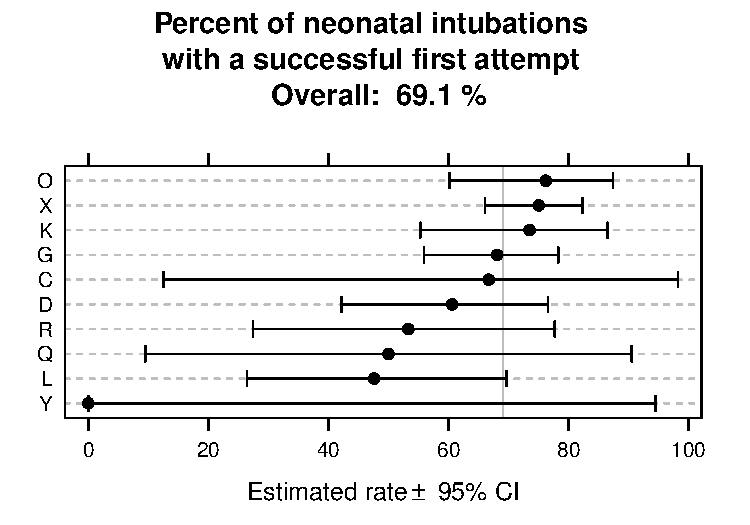
\includegraphics[width=\maxwidth]{figure/r_neonatal_intubation_success} 

\end{knitrout}

\end{center}

% latex table generated in R 3.0.2 by xtable 1.7-1 package
% Fri May 30 21:10:44 2014
\begin{table}[ht]
\centering
\begin{tabular}{lrrrrr}
  \hline
Program & den. & num. & lower CI & rate & upper CI \\ 
  \hline
O & 42.0 & 32.0 & 60.2 & 76.2 & 87.4 \\ 
  X & 120.0 & 90.0 & 66.1 & 75.0 & 82.3 \\ 
  K & 34.0 & 25.0 & 55.3 & 73.5 & 86.5 \\ 
  G & 72.0 & 49.0 & 55.9 & 68.1 & 78.3 \\ 
  C & 3.0 & 2.0 & 12.5 & 66.7 & 98.2 \\ 
  D & 33.0 & 20.0 & 42.2 & 60.6 & 76.6 \\ 
  R & 15.0 & 8.0 & 27.4 & 53.3 & 77.7 \\ 
  Q & 2.0 & 1.0 & 9.5 & 50.0 & 90.5 \\ 
  L & 21.0 & 10.0 & 26.4 & 47.6 & 69.7 \\ 
  Y & 1.0 & 0.0 & 0.0 & 0.0 & 94.5 \\ 
   \hline
\end{tabular}
\end{table}




\newpage
\subsection{Pediatric: First attempt tracheal tube placement success}
The total number of intubations successful on the first attempt DIVIDED by the number of patients on whom intubation was attempted by the transport team during the calendar month. "Intubation attempt" is further defined as laryngoscopy by any member of the transport team regardless of whether there is an attempt to pass a tracheal tube. A successful intubation is further defined as that which has ben confmrimed as described in "Verification of TT tube placement." First-attempt success should not be disqualified by necessary adjustments to the depth of the TT and re-securing it. Includes patients older than than 28 days (non-neonates).

\begin{center}
\begin{knitrout}
\definecolor{shadecolor}{rgb}{0.969, 0.969, 0.969}\color{fgcolor}
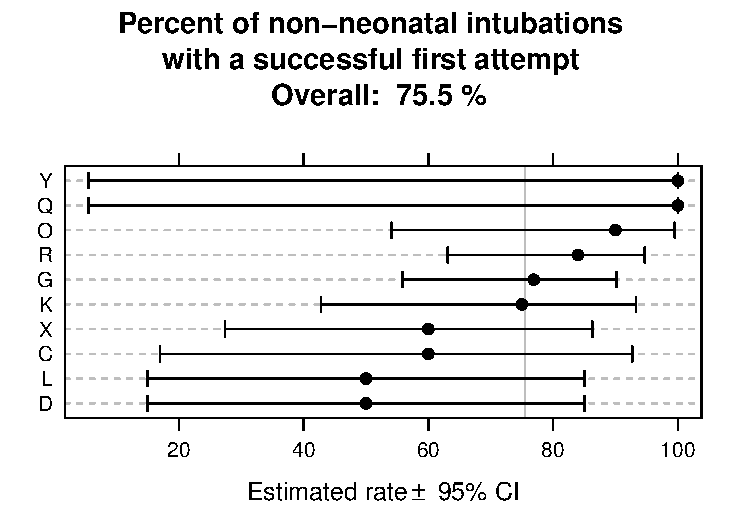
\includegraphics[width=\maxwidth]{figure/r_pediatric_intubation_success} 

\end{knitrout}

\end{center}

% latex table generated in R 3.0.2 by xtable 1.7-1 package
% Fri May 30 21:10:44 2014
\begin{table}[ht]
\centering
\begin{tabular}{lrrrrr}
  \hline
Program & den. & num. & lower CI & rate & upper CI \\ 
  \hline
Q & 1.0 & 1.0 & 5.5 & 100.0 & 100.0 \\ 
  Y & 1.0 & 1.0 & 5.5 & 100.0 & 100.0 \\ 
  O & 10.0 & 9.0 & 54.1 & 90.0 & 99.5 \\ 
  R & 25.0 & 21.0 & 63.1 & 84.0 & 94.7 \\ 
  G & 26.0 & 20.0 & 55.9 & 76.9 & 90.2 \\ 
  K & 12.0 & 9.0 & 42.8 & 75.0 & 93.3 \\ 
  X & 10.0 & 6.0 & 27.4 & 60.0 & 86.3 \\ 
  C & 5.0 & 3.0 & 17.0 & 60.0 & 92.7 \\ 
  D & 4.0 & 2.0 & 15.0 & 50.0 & 85.0 \\ 
  L & 4.0 & 2.0 & 15.0 & 50.0 & 85.0 \\ 
   \hline
\end{tabular}
\end{table}






\newpage
\section{Operational metrics}
\subsection{Use of a standardized patient-care handoff}
The number of transports for which there is documented use of a standardized hand-off procedure for turning over patient care at the destination hospital DIVIDED by the number of transports during the calendar month.

\begin{center}
\begin{knitrout}
\definecolor{shadecolor}{rgb}{0.969, 0.969, 0.969}\color{fgcolor}
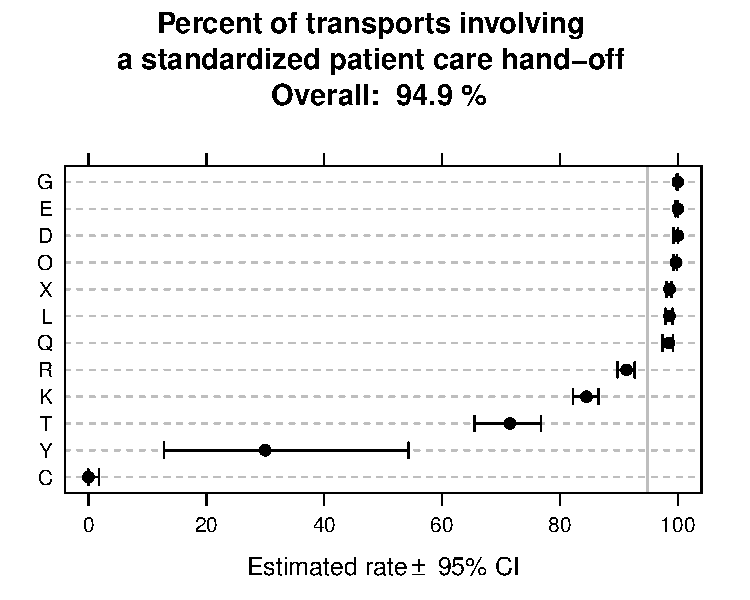
\includegraphics[width=\maxwidth]{figure/r_standardized_handoff} 

\end{knitrout}

\end{center}

% latex table generated in R 3.0.2 by xtable 1.7-1 package
% Fri May 30 21:10:44 2014
\begin{table}[ht]
\centering
\begin{tabular}{lrrrrr}
  \hline
Program & den. & num. & lower CI & rate & upper CI \\ 
  \hline
G & 1994.0 & 1994.0 & 99.8 & 100.0 & 100.0 \\ 
  E & 1061.0 & 1061.0 & 99.6 & 100.0 & 100.0 \\ 
  D & 651.0 & 651.0 & 99.3 & 100.0 & 100.0 \\ 
  O & 2025.0 & 2019.0 & 99.3 & 99.7 & 99.9 \\ 
  X & 3318.0 & 3270.0 & 98.1 & 98.6 & 98.9 \\ 
  L & 1665.0 & 1642.0 & 97.9 & 98.6 & 99.1 \\ 
  Q & 884.0 & 871.0 & 97.4 & 98.5 & 99.2 \\ 
  R & 1521.0 & 1389.0 & 89.8 & 91.3 & 92.7 \\ 
  K & 1184.0 & 1000.0 & 82.2 & 84.5 & 86.5 \\ 
  T & 256.0 & 183.0 & 65.5 & 71.5 & 76.8 \\ 
  Y & 20.0 & 6.0 & 12.8 & 30.0 & 54.3 \\ 
  C & 264.0 & 0.0 & 0.0 & 0.0 & 1.8 \\ 
   \hline
\end{tabular}
\end{table}



\newpage
\subsection{Average mobilization time of the transport team}
The average time (includes all transports in the calendar month, excluding transports scheduled in advance and patient transports out of the originating facility) in minutes (rounded up to nearest minute) from the start of the referral phone call to the transport team to the time the transport team is en route to the referral facility. "Stacked" trips or transports right after the last during which the team never returns to base should still be included in this count.

\let\thefootnote\relax\footnote{Average time weighted by monthly run volume.}

\begin{center}
\begin{knitrout}
\definecolor{shadecolor}{rgb}{0.969, 0.969, 0.969}\color{fgcolor}
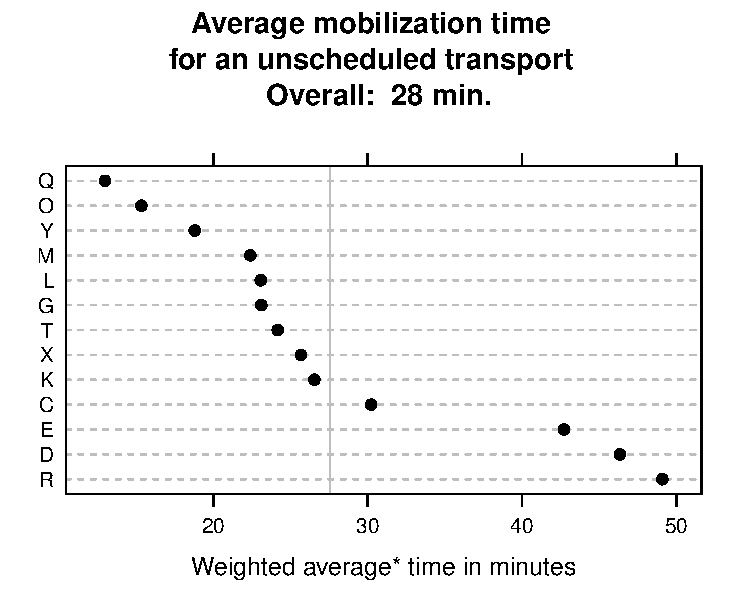
\includegraphics[width=\maxwidth]{figure/r_mobilization_time} 

\end{knitrout}

\end{center}







\newpage
\section{Safety metrics}
\subsection{Rate of patient medical equipment failure during transport}
The number of documented medical equipment failures (may be more than 1 per transport) while under the care of the transport team DIVIDED by the number of transports during the calendar month. Examples include IV pumps and ventilators that malfunction during transport, broken monitor leads, empty medical gas tanks, etc.

\begin{center}
\begin{knitrout}
\definecolor{shadecolor}{rgb}{0.969, 0.969, 0.969}\color{fgcolor}
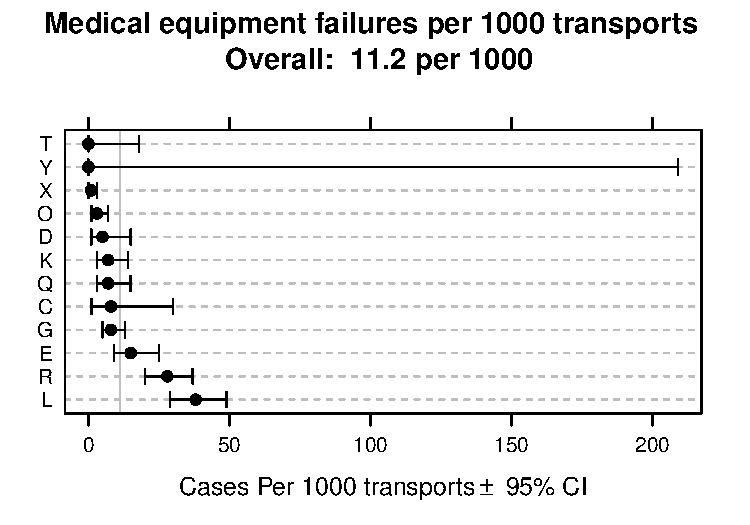
\includegraphics[width=\maxwidth]{figure/r_med_equip_failure} 

\end{knitrout}

\end{center}

% latex table generated in R 3.0.2 by xtable 1.7-1 package
% Fri May 30 21:10:45 2014
\begin{table}[ht]
\centering
\begin{tabular}{lrrrrr}
  \hline
Program & den. & num. & lower CI & rate & upper CI \\ 
  \hline
T & 256.0 & 0.0 & 0.0 & 0.0 & 18.0 \\ 
  Y & 19.0 & 0.0 & 0.0 & 0.0 & 209.0 \\ 
  X & 3300.0 & 4.0 & 0.0 & 1.0 & 3.0 \\ 
  O & 2019.0 & 6.0 & 1.0 & 3.0 & 7.0 \\ 
  D & 637.0 & 3.0 & 1.0 & 5.0 & 15.0 \\ 
  K & 1159.0 & 8.0 & 3.0 & 7.0 & 14.0 \\ 
  Q & 884.0 & 6.0 & 3.0 & 7.0 & 15.0 \\ 
  C & 264.0 & 2.0 & 1.0 & 8.0 & 30.0 \\ 
  G & 1994.0 & 16.0 & 5.0 & 8.0 & 13.0 \\ 
  E & 1061.0 & 16.0 & 9.0 & 15.0 & 25.0 \\ 
  R & 1521.0 & 42.0 & 20.0 & 28.0 & 37.0 \\ 
  L & 1663.0 & 63.0 & 29.0 & 38.0 & 49.0 \\ 
   \hline
\end{tabular}
\end{table}




\newpage
\subsection{Rate of transport-related patient injuries}
The number of documented transport-related patient injuries or deaths DIVIDED by the number of transports during the calendar month. Excluded are injuries and deaths related to the medical care itself or the omission of medical care. Examples include a patient fall, a loose piece of transport equipment that falls and strikes the patient, injury suffered in a transport vehicle accident, etc.

\begin{center}
\begin{knitrout}
\definecolor{shadecolor}{rgb}{0.969, 0.969, 0.969}\color{fgcolor}
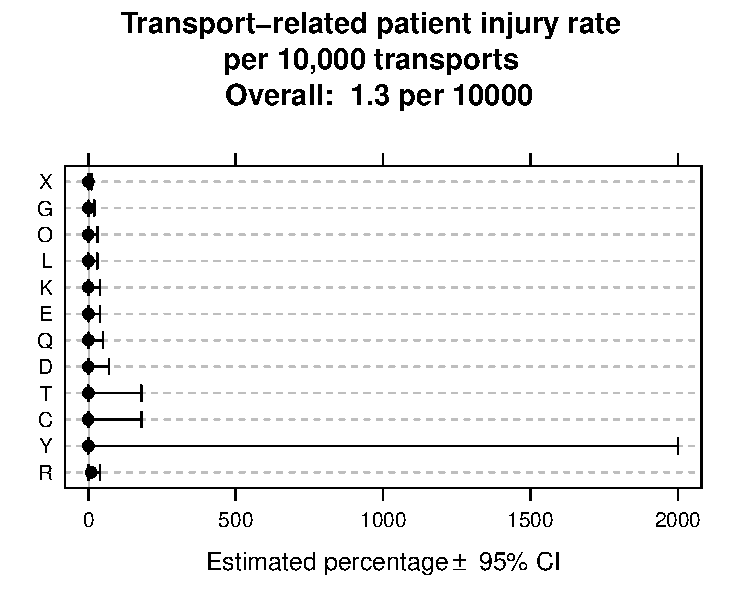
\includegraphics[width=\maxwidth]{figure/r_patient_injuries} 

\end{knitrout}

\end{center}

% latex table generated in R 3.0.2 by xtable 1.7-1 package
% Fri May 30 21:10:45 2014
\begin{table}[ht]
\centering
\begin{tabular}{lrrrrr}
  \hline
Program & den. & num. & lower CI & rate & upper CI \\ 
  \hline
X & 3318.0 & 0.0 & 0.0 & 0.0 & 10.0 \\ 
  G & 1994.0 & 0.0 & 0.0 & 0.0 & 20.0 \\ 
  L & 1665.0 & 0.0 & 0.0 & 0.0 & 30.0 \\ 
  O & 2025.0 & 1.0 & 0.0 & 0.0 & 30.0 \\ 
  E & 1061.0 & 0.0 & 0.0 & 0.0 & 40.0 \\ 
  K & 1184.0 & 0.0 & 0.0 & 0.0 & 40.0 \\ 
  Q & 884.0 & 0.0 & 0.0 & 0.0 & 50.0 \\ 
  D & 651.0 & 0.0 & 0.0 & 0.0 & 70.0 \\ 
  C & 264.0 & 0.0 & 0.0 & 0.0 & 180.0 \\ 
  T & 256.0 & 0.0 & 0.0 & 0.0 & 180.0 \\ 
  Y & 20.0 & 0.0 & 0.0 & 0.0 & 2000.0 \\ 
  R & 1521.0 & 1.0 & 0.0 & 10.0 & 40.0 \\ 
   \hline
\end{tabular}
\end{table}




\newpage
\subsection{Rate of transport-related crew injuries}
The number of transport-related crew injuries or deaths reported to the institution's employee health department or equivalent during the calendar month DIVIDED by the number of transports during the calendar month.

\begin{center}
\begin{knitrout}
\definecolor{shadecolor}{rgb}{0.969, 0.969, 0.969}\color{fgcolor}
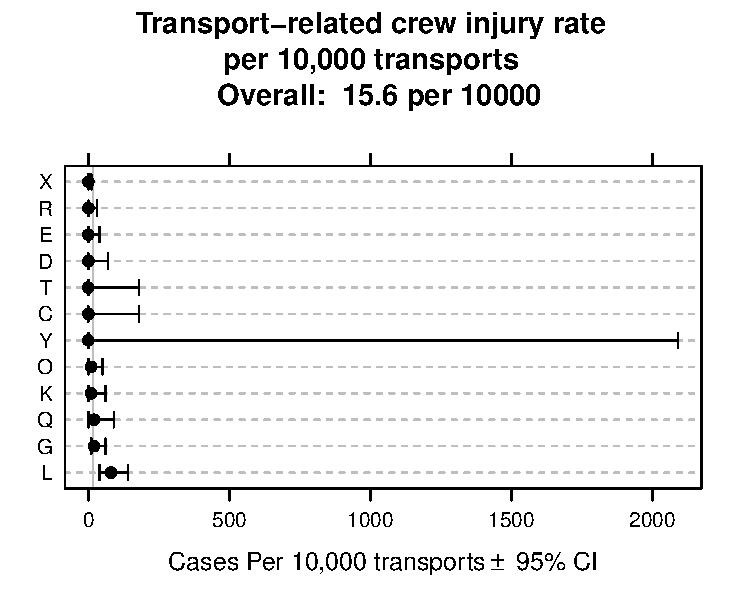
\includegraphics[width=\maxwidth]{figure/r_crew_injuries} 

\end{knitrout}

\end{center}

% latex table generated in R 3.0.2 by xtable 1.7-1 package
% Fri May 30 21:10:45 2014
\begin{table}[ht]
\centering
\begin{tabular}{lrrrrr}
  \hline
Program & den. & num. & lower CI & rate & upper CI \\ 
  \hline
X & 3300.0 & 0.0 & 0.0 & 0.0 & 10.0 \\ 
  R & 1521.0 & 0.0 & 0.0 & 0.0 & 30.0 \\ 
  E & 1061.0 & 0.0 & 0.0 & 0.0 & 40.0 \\ 
  D & 637.0 & 0.0 & 0.0 & 0.0 & 70.0 \\ 
  C & 264.0 & 0.0 & 0.0 & 0.0 & 180.0 \\ 
  T & 256.0 & 0.0 & 0.0 & 0.0 & 180.0 \\ 
  Y & 19.0 & 0.0 & 0.0 & 0.0 & 2090.0 \\ 
  O & 2019.0 & 3.0 & 0.0 & 10.0 & 50.0 \\ 
  K & 1159.0 & 1.0 & 0.0 & 10.0 & 60.0 \\ 
  Q & 884.0 & 2.0 & 0.0 & 20.0 & 90.0 \\ 
  G & 1994.0 & 4.0 & 10.0 & 20.0 & 60.0 \\ 
  L & 1663.0 & 13.0 & 40.0 & 80.0 & 140.0 \\ 
   \hline
\end{tabular}
\end{table}



\newpage
\section{Rare Events}
\subsection{Rate of medication administration errors}
The number of documented medication administration errors during a calendar month DIVIDED by the number of transports during the calendar month. Medication administration errors are further defined as drug admnistrations violating any of the "five-rights" -- right patient, right medication, right dose, right route, and right time.

\begin{center}
\begin{knitrout}
\definecolor{shadecolor}{rgb}{0.969, 0.969, 0.969}\color{fgcolor}
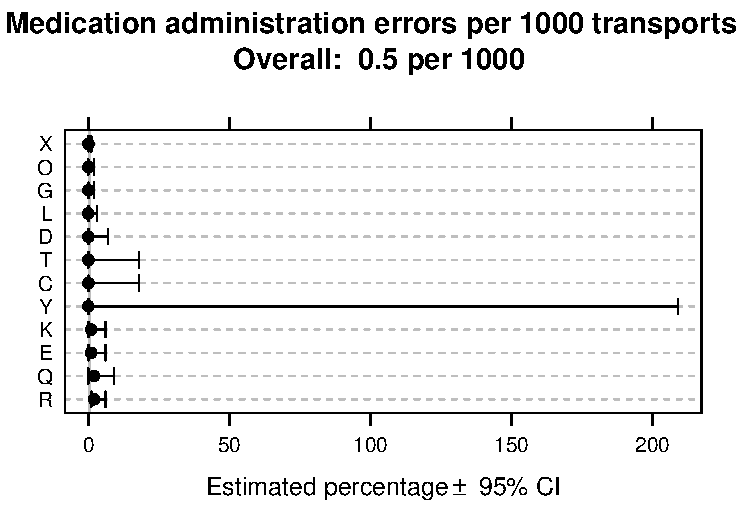
\includegraphics[width=\maxwidth]{figure/r_med_errors} 

\end{knitrout}

\end{center}

% latex table generated in R 3.0.2 by xtable 1.7-1 package
% Fri May 30 21:10:45 2014
\begin{table}[ht]
\centering
\begin{tabular}{lrrrrr}
  \hline
Program & den. & num. & lower CI & rate & upper CI \\ 
  \hline
X & 3300.0 & 0.0 & 0.0 & 0.0 & 1.0 \\ 
  G & 1994.0 & 0.0 & 0.0 & 0.0 & 2.0 \\ 
  O & 2019.0 & 0.0 & 0.0 & 0.0 & 2.0 \\ 
  L & 1663.0 & 0.0 & 0.0 & 0.0 & 3.0 \\ 
  D & 637.0 & 0.0 & 0.0 & 0.0 & 7.0 \\ 
  C & 264.0 & 0.0 & 0.0 & 0.0 & 18.0 \\ 
  T & 256.0 & 0.0 & 0.0 & 0.0 & 18.0 \\ 
  Y & 19.0 & 0.0 & 0.0 & 0.0 & 209.0 \\ 
  E & 1061.0 & 1.0 & 0.0 & 1.0 & 6.0 \\ 
  K & 1159.0 & 1.0 & 0.0 & 1.0 & 6.0 \\ 
  Q & 884.0 & 2.0 & 0.0 & 2.0 & 9.0 \\ 
  R & 1521.0 & 3.0 & 1.0 & 2.0 & 6.0 \\ 
   \hline
\end{tabular}
\end{table}




\newpage
\subsection{Rate of CPR performed during transport}
The number of transports during which chest compressions are performed from the time the transport team assumes care ("hands on") until the patient hand-off is completed at the destination facility DIVIDED by the number of transports during the calendar month. Multiple episodes of chest compressions in a single transport should only be counted as one episode. If CPR is in progress when the team arrives, this should not be included in this count.

\begin{center}
\begin{knitrout}
\definecolor{shadecolor}{rgb}{0.969, 0.969, 0.969}\color{fgcolor}
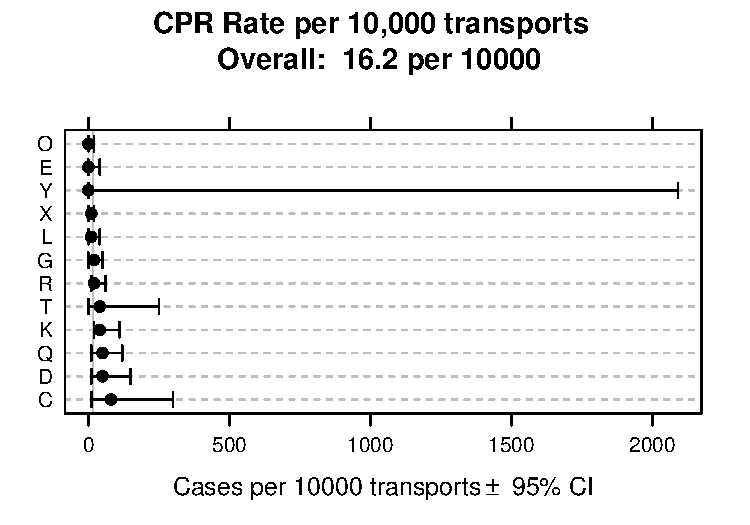
\includegraphics[width=\maxwidth]{figure/r_cpr} 

\end{knitrout}

\end{center}

% latex table generated in R 3.0.2 by xtable 1.7-1 package
% Fri May 30 21:10:46 2014
\begin{table}[ht]
\centering
\begin{tabular}{lrrrrr}
  \hline
Program & den. & num. & lower CI & rate & upper CI \\ 
  \hline
O & 2019.0 & 0.0 & 0.0 & 0.0 & 20.0 \\ 
  E & 1061.0 & 0.0 & 0.0 & 0.0 & 40.0 \\ 
  Y & 19.0 & 0.0 & 0.0 & 0.0 & 2090.0 \\ 
  X & 3300.0 & 2.0 & 0.0 & 10.0 & 20.0 \\ 
  L & 1663.0 & 1.0 & 0.0 & 10.0 & 40.0 \\ 
  G & 1994.0 & 3.0 & 0.0 & 20.0 & 50.0 \\ 
  R & 1521.0 & 3.0 & 10.0 & 20.0 & 60.0 \\ 
  T & 256.0 & 1.0 & 0.0 & 40.0 & 250.0 \\ 
  K & 1159.0 & 5.0 & 20.0 & 40.0 & 110.0 \\ 
  Q & 884.0 & 4.0 & 10.0 & 50.0 & 120.0 \\ 
  D & 637.0 & 3.0 & 10.0 & 50.0 & 150.0 \\ 
  C & 264.0 & 2.0 & 10.0 & 80.0 & 300.0 \\ 
   \hline
\end{tabular}
\end{table}




\newpage
\subsection{Rate of Serious Reportable Events (SREs)}
The number of SREs during the calendar month DIVIDED by the number of transports during the calendar month. An SRE is defined as any unanticipated and largely preventable event involving death, life-threatening consequences, or serious physical or psychological harm. Qualifying events include but are not limited to the National Quality Forum's Serious Reportable Events available at \url{http://www.qualityforum.org/Topics/SREs/List_of_SREs.aspx}.

\begin{center}
\begin{knitrout}
\definecolor{shadecolor}{rgb}{0.969, 0.969, 0.969}\color{fgcolor}
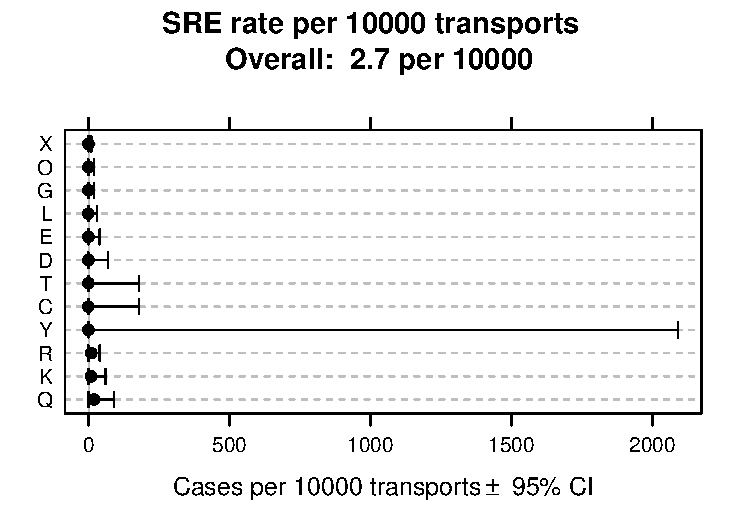
\includegraphics[width=\maxwidth]{figure/r_SRE} 

\end{knitrout}

\end{center}

% latex table generated in R 3.0.2 by xtable 1.7-1 package
% Fri May 30 21:10:46 2014
\begin{table}[ht]
\centering
\begin{tabular}{lrrrrr}
  \hline
Program & den. & num. & lower CI & rate & upper CI \\ 
  \hline
X & 3300.0 & 0.0 & 0.0 & 0.0 & 10.0 \\ 
  G & 1994.0 & 0.0 & 0.0 & 0.0 & 20.0 \\ 
  O & 2019.0 & 0.0 & 0.0 & 0.0 & 20.0 \\ 
  L & 1663.0 & 0.0 & 0.0 & 0.0 & 30.0 \\ 
  E & 1061.0 & 0.0 & 0.0 & 0.0 & 40.0 \\ 
  D & 637.0 & 0.0 & 0.0 & 0.0 & 70.0 \\ 
  C & 264.0 & 0.0 & 0.0 & 0.0 & 180.0 \\ 
  T & 256.0 & 0.0 & 0.0 & 0.0 & 180.0 \\ 
  Y & 19.0 & 0.0 & 0.0 & 0.0 & 2090.0 \\ 
  R & 1521.0 & 1.0 & 0.0 & 10.0 & 40.0 \\ 
  K & 1159.0 & 1.0 & 0.0 & 10.0 & 60.0 \\ 
  Q & 884.0 & 2.0 & 0.0 & 20.0 & 90.0 \\ 
   \hline
\end{tabular}
\end{table}




\newpage




\end{center}
\end{document}
